WFS theory is based on a propagation model where the acoustic field is generated by punctual primary sources and the cancellation field is generated by punctual monopole secondary sources, everything in an homogeneous media and free-space condition, and the location of every source is perfectly known.

A real situation, as the one we find in a listening room with real loudspeakers, is very different. A great variety of phenomena not contemplated by the WFS simple model occur: reflections, diffractions produced by obstacles, loudspeakers are not punctual sources so the near-field does not follow the far-field approximation, the directivity is not the one of an ideal monopole and depends on the frequency, the frequency response of loudspeakers is not flat, which would not be that big of a problem if it was the same for every loudspeaker, but it might actually be very different from one to the other, their exact locations are not accurately known, non-linearities, etc.

All these differences influence the way the acoustic waves propagate and, in general, they worsen the performance in a real situation. Experimental measures help us understand how this not contemplated differences limit the possibilities of using WFS in the real world.
\begin{shownto}{private}
\section{Acoustic path model}
In order to find a connection between the real and ideal situation, let's use a model of what is happening.
\end{shownto}
In a real situation, all we can certainly know is that, if we transmit a signal through a loudspeaker and we measure at some point with a microphone, we receive a modified version of the signal. That modification depends on all the conditions previously mentioned (multiple reflections, etc.), and together they form what is often called acoustic path. An acoustic path between a loudspeaker and a point of measure acts as a filter characterized by an impulse response (time domain) or frequency response (frequency domain).

When we use $\numWFS$ secondary loudspeakers, $\numNS$ noise sources and $\numMeasPoints$ points of measure, the relation between transmitted signals and received ones in the frequency domain is:
\begin{shownto}{private}
\begin{equation}
\Field[noValue][frequency][vector](f) = \AcPath[mat](f) \vec{\signal[nothing][frequency]}(f) ,
\end{equation}
where $\Field[noValue][frequency][vector] = [\Field[noValue][frequency][scalar]_1, \Field[noValue][frequency][scalar]_2, ..., \Field[noValue][frequency][scalar]_\numMeasPoints]^T$ ($\numMeasPoints$ is the number of points of measure) is the acoustic pressure vector, $\vec{\signal[nothing][frequency]} = [\signal[nothing][frequency]_1, \signal[nothing][frequency]_2, ..., \signal[nothing][frequency]_\numSources]^T$ ($\numSources$ is the number of loudspeakers) is the transmitted signals vector, and $\AcPath[mat]_{(\numMeasPoints \times \numSources)}$ is a matrix whose $(m,n)$-th element is the frequency response of the acoustic path between the $n$-th loudspeaker and the $m$-th point of measure.

When we differentiate the noise sources and the WFS array sources:
\begin{multline}
\Field[noValue][frequency][vector](f)
= \left. \begin{cases}
\vec{\signal[nothing][frequency]} = 
\begin{bmatrix}
\vec{\signal[wfs][frequency]} \\
\vec{\signal[ns][frequency]}
\end{bmatrix} \\
\AcPath[mat] =
\begin{bmatrix}
\AcPath[mat][WFS], & \AcPath[mat][NS]
\end{bmatrix}
\end{cases} \right\} \\
 = \AcPath[mat][NS](f) \vec{\signal[ns][frequency]}(f) + \AcPath[mat][WFS](f) \vec{\signal[wfs][frequency]}(f)
 = \Field[ns][frequency][vector](f) + \Field[wfs][frequency][vector](f),
\end{multline}
where $\Field[ns][frequency][vector] = [\Field[ns][frequency][scalar][1], \Field[ns][frequency][scalar][2], ..., \Field[ns][frequency][scalar][\numMeasPoints]]^T$, $\Field[wfs][frequency][vector] = [\Field[wfs][frequency][scalar][1], \Field[wfs][frequency][scalar][2], ..., \Field[wfs][frequency][scalar][\numMeasPoints]]^T$, $\vec{\signal[ns][frequency]} = [\signal[ns][frequency]_1, \signal[ns][frequency]_2, ..., \signal[ns][frequency]_{\numNS}]^T$ ($\numNS$ is the number of noise sources), $\vec{\signal[wfs][frequency]} = [\signal[wfs][frequency]_1, \signal[wfs][frequency]_2, ..., \signal[wfs][frequency]_{\numWFS}]^T$ ($\numWFS$ is the number of secondary sources) and $\AcPath[mat][NS]$ and $\AcPath[mat][WFS]$ are the acoustic path matrices of the noise sources and WFS secondary source array respectively. If the cancellation is successful, $\Field[ns][frequency][vector](f) \approx -\Field[wfs][frequency][vector](f)$ and so, $\Field[noValue][frequency][vector]$ becomes really small.
\end{shownto}

\begin{shownto}{public}
\begin{multline}
	\Field[noValue][frequency][vector](f)
	= \AcPath[mat](f) \vec{\signal[nothing][frequency]}(f)
	= \left. \begin{cases}
		\vec{\signal[nothing][frequency]} = 
		\begin{bmatrix}
			\vec{\signal[wfs][frequency]} \\
			\vec{\signal[ns][frequency]}
		\end{bmatrix} \\
		\AcPath[mat] =
		\begin{bmatrix}
			\AcPath[mat][WFS], & \AcPath[mat][NS]
		\end{bmatrix}
	\end{cases} \right\} \\
	= \AcPath[mat][NS](f) \vec{\signal[ns][frequency]}(f) + \AcPath[mat][WFS](f) \vec{\signal[wfs][frequency]}(f)
	= \Field[ns][frequency][vector](f) + \Field[wfs][frequency][vector](f),
	\label{acPathModel}
\end{multline}
where $\Field[ns][frequency][vector] = [\Field[ns][frequency][scalar][1], \Field[ns][frequency][scalar][2], ..., \Field[ns][frequency][scalar][\numMeasPoints]]^T$ and $\Field[wfs][frequency][vector] = [\Field[wfs][frequency][scalar][1], \Field[wfs][frequency][scalar][2], ..., \Field[wfs][frequency][scalar][\numMeasPoints]]^T$ are the acoustic pressure vectors ($\numMeasPoints$ is the number of points of measure), $\vec{\signal[ns][frequency]} = [\signal[ns][frequency]_1, \signal[ns][frequency]_2, ..., \signal[ns][frequency]_{\numNS}]^T$ ($\numNS$ is the number of noise sources) and $\vec{\signal[wfs][frequency]} = [\signal[wfs][frequency]_1, \signal[wfs][frequency]_2, ..., \signal[wfs][frequency]_{\numWFS}]^T$ ($\numWFS$ is the number of secondary sources) are the transmitted signal vectors, and ${\AcPath[mat][NS]}_{(\numMeasPoints \times \numNS)}$ and ${\AcPath[mat][WFS]}_{(\numMeasPoints \times \numWFS)}$ are matrices whose $(m,n)$-th element is the frequency response of the acoustic path between the $n$-th loudspeaker and the $m$-th point of measure. If the cancellation is successful, $\Field[ns][frequency][vector](f) \approx -\Field[wfs][frequency][vector](f)$ and so, the elements of $\Field[noValue][frequency][vector]$ become really small. Cancellation will be successful as long as the acoustic paths are the same or very similar to the ideal ones. In the ideal case, the $(m,n)$-th element of $\AcPath$ would apply a simple delay and an amplitude attenuation:
\begin{equation}
a_{m,n}(f) = \frac{e^{-j k d_{m,n}}}{d_{m,n}},
\end{equation}
where $d_{m,n}$ is the distance between the $n$-th loudspeaker and the $m$-th point of measure.
\end{shownto}

\begin{shownto}{private}
The signal reproduced by the secondary loudspeakers $\vec{\signal[wfs][frequency]}$ depends on the noise source signals $\vec{\signal[ns][frequency]}$. Specifically, each secondary source filters the noise source signals, as it was expressed in \autoref{rayleigh2_5Dsignal} and rewritten here:
\begin{multline}
\signal[wfs][frequency](f) = \signal[nsVirt][frequency](f) \frac{g \cos\normPrimaryPropAngleSection}{\sqrt{\distLinePrimSource}}
e^{-j k \distLinePrimSource} \sqrt{\frac{jk}{2\pi}} = \\
\left\{
\signal[nsVirt][frequency](f) = -\signal[ns][frequency] \rightarrow
H(f) = -\frac{g \cos\normPrimaryPropAngleSection}{\sqrt{\distLinePrimSource}}
e^{-j k \distLinePrimSource} \sqrt{\frac{jk}{2\pi}}
\right\} = \signal[ns][frequency](f) H(f).
\end{multline}
Expressed as a matrix multiplication:
\begin{equation}
\vec{\signal[wfs][frequency]} = \myMatrix{H} \vec{\signal[ns][frequency]},
\end{equation}
where $\myMatrix{H}_{\numWFS \times \numNS}(f)$ is a matrix where the $(m,n)$-th element is the filter frequency response that the $m$-th array loudspeaker applies to the $n$-th noise source.

In the model assumed by WFS theory (free-space conditions, ideal monopole point sources), the acoustic path response between a source and a point of measure separated by a distance $d$ is:
\begin{equation}
a(f) = \frac{e^{-j k d}}{d}.
\end{equation}
This allows us to construct $\AcPath[mat]'(f)$, the acoustic path response matrix for ideal conditions. The $(m,n)$-th element would be 
\begin{equation}
a_{m,n}'(f) = \frac{e^{-j k d_{m,n}}}{d_{m,n}},
\end{equation}
where $d_{m,n}$ is the distance between the $n$-th loudspeaker and the $m$-th point of measure.

Under these conditions, good cancellation levels can be achieved. The actual $\AcPath[mat]$ includes all sorts of variations, as we saw, so one could expect the experimental result to be much worse than what theory predicts.
\end{shownto}

\begin{shownto}{private}
\section{Volume correction}
However, a way of making this model more realistic is by adding a variable that accounts for the possible sound volume difference between the noise source and the secondary loudspeaker array. This is useful because in the listening room we generate the noise signal with a loudspeaker. Unlike the secondary array loudspeakers, which were all adjusted to have similar behaviour, the noise loudspeaker volume can be independently adjusted manually. If we change it for another loudspeaker, the volume might be actually very different. This introduces an unknown variable that definitely affects cancellation, but it's really easy to model and compensate.

Basically, regarding the volume of the source as a separate variable when dealing with real loudspeakers, force us to differentiate between the digital signal in arbitrary units $\signal[nothing][frequency]$, and the real signal in acoustic pressure units (for example, Pascals) $\soundVolume \signal[nothing][frequency]$, where $\soundVolume$ is the sound volume of the loudspeaker that transforms arbitrary units in pressure units. This term goes then included in the acoustic path matrix $\AcPath[mat]$, where the $n$-th column is multiplied by the volume associated to the $n$-th loudspeaker. Since we consider that all loudspeakers of the secondary array are well calibrated and, for simplification purposes, also considering all noise loudspeakers have the same volume:
\begin{equation}
\Field[noValue][frequency][vector]
= (\soundVolume[ns]\AcPath[mat][NS]' + \soundVolume[wfs]\AcPath[mat][WFS]'\myMatrix{H}) \vec{\signal[ns][frequency]},
\end{equation}
where $\AcPath[mat][NS]'$ and $\AcPath[mat][WFS]'$ are the ideal acoustic path matrices when the volume term is not included. This means that $\AcPath[mat][NS] = \soundVolume[ns]\AcPath[mat][NS]'$ and $\AcPath[mat][WFS] = \soundVolume[wfs]\AcPath[mat][WFS]'$.

In order to perform cancellation, we must compensate for this volume difference by multiplying the amplitude of cancellation signals by $\globalCorrectionFactor = \soundVolume[ns]/\soundVolume[wfs]$. It can be estimated after measures or if we know the acoustic path responses by finding, for example, the real number $\correctionFactor$ that optimizes next expression:
\begin{equation}
\globalCorrectionFactor = \min_\correctionFactor \norm{\Field[wfs][frequency][vector]\correctionFactor + \Field[ns][frequency][vector]}^2 = \min_\correctionFactor \norm{(\AcPath[mat][NS] + \AcPath[mat][WFS]\myMatrix{H}\correctionFactor)\vec{\signal[ns][frequency]}}^2 = -\frac{\Re\left(\scalarProd{\Field[wfs][frequency][vector]^*}{\Field[ns][frequency][vector]}\right)}{\norm{\Field[wfs][frequency][vector]}^2}
\end{equation}
In a way, this is like finding the virtual noise source signal $\vec{\signal[nsVirt][frequency]}$ that maximizes cancellation, with the restriction that it must be a scaled version of of $\vec{\signal[ns][frequency]}$.
It is not the only way we can experimentally estimate this number, but it is a simple and useful way. By compensating the volume difference, at least we can measure WFS performance as if no volume difference was present.
\end{shownto}

\begin{shownto}{private}
\section{Justification for optimization}
The extent of the optimization depends on what we want to test. If we only wanted to test how much unpredictable variables affect performance, counting volume disparity as one of those variables, it would not make sense to perform an optimization, because it would be falsifying the results. However, if we consider the volume disparity as a problem inherent to the listening room situation and not a general one, or that in a more real situation it can be solved, or optimized in real-time, then it makes sense to optimize. Hence, it is important to define what we want to test.

We have considered that, in order to fairly assess WFS performance, the volume disparity shouldn't be something the WFS technique must solve. We want to know its possibilities given that the strength of the noise source is known, this is, that the system of microphones that measure noise strength, no matter they are situated close to the secondary sources or to the noise source (depending on the architecture of the actual setup), provides the WFS algorithm with a good estimation of signal strength. So it is fair, and even necessary, to correct for volume disparity in the laboratory, since we assume that in the real situation it would be a solved problem. Even if it is not, in a real situation we can also optimize a posteriori based on measures in the sound cancellation area. Anyway one wants to describe a real situation, the point is that WFS technique is not responsible for wrong estimations of primary source signal strength; that is a problem that must be solved with other techniques available. The described optimization is, indeed, one of those techniques.

Other variables as reflections, diffractions, etc., shouldn't be compensated because there is actually where we can see the effectiveness of WFS in front of real situations where acoustic paths are unpredictable. For example, achieving silence on a small number of microphones is easy by solving the linear system, but it's not WFS, it's a completely different technique that does not guarantee sound cancellation over the whole area.
\end{shownto}

\begin{shownto}{private}
\section{Acoustic path frequency response estimation}
In order to measure the acoustic path frequency response, we have used a simple algorithm that can easily be implemented in Matlab.

If we were only to calculate the acoustic path between a source and one or multiple microphones, it would be actually pretty easy.

...

However, the number of sources in the listening room is 96. It is a large number, and it would be convenient to find a better, fastest way of calculating it. The technique we have used is based on orthogonal frequency division multiplexing, this is, the fact that each loudspeaker transmits different, orthogonal frequencies that can be easily separated in the received signal.

In a communication system, a signal $x(t)$ gets transmitted through a channel with impulse response $h(t)$, and the received signal $y(t)$ is the convolution of the previous two:
\begin{equation}
y(t) = x(t)\ast h(t)
\end{equation}

Generally, in practical situations we can consider that $h(t)$ is causal and limited in time, with a duration $T_h$:
\begin{equation}
h(t) = h(t) \Pi\left(\frac{t - T_h/2}{T_h}\right)
\end{equation}
where $\Pi(t)$ is the rectangular function
\begin{equation}
\Pi(t) = \mathit{rect}(t) = \begin{cases}
0, & t < -1/2 \\
1, & -1/2 < t < 1/2 \\
0, & 1/2 < t
\end{cases}
\end{equation}

This implies that if we are only interested in knowing $y(t)$ in an interval $t \in [t_\mathit{ini}, t_\mathit{end}]$, then we just need to know $x(t)$ in the interval $t \in [t_\mathit{ini} - T_h, t_\mathit{end}]$:
\begin{equation}
y(t) = \Pi\left(\frac{t - (t_\mathit{end} + t_\mathit{ini} - T_h)/2}{t_\mathit{end} - (t_\mathit{ini} - T_h)}\right) x(t) \ast h(t), \quad t_\mathit{ini} <= t <= t_\mathit{end}.
\end{equation}

The spectrum of that interval of the received signal will be
\begin{multline}
Y'(f) = \FourierTransform{y'(t)} = \FourierTransform{y(t) \Pi\left(\frac{t - (t_\mathit{end} + t_\mathit{end})/2}{t_\mathit{end} - t_\mathit{ini}}\right)} = \\ Y(f) \ast (t_\mathit{end} - t_\mathit{ini}) \sinc\left((t_\mathit{end} - t_\mathit{ini}) f \right) e^{-j 2 \pi f \frac{(t_\mathit{end} + t_\mathit{ini})}{2}},
\end{multline}
where $\mathit{sinc}$ is the function:
\begin{equation}
\sinc(x) = \frac{\sin(\pi x)}{\pi x}
\end{equation}

Let's assume that we are transmitting some tones with equispaced frequencies $f_k = k \Delta f$, where $k = -N - 1, ..., 0, ..., N-1$ ($x(t)$ is real). As a consequence, if the duration of the selected interval of $y(t)$ is multiple of $1/\Delta f$, this is, $T = t_\mathit{end} - t_\mathit{ini} = n/\Delta f$ where $n = 1, 2, ...$, then the zeroes of the $\mathit{sinc}$ function fall on multiples of $1/T = \Delta f / n$, meaning that 
\begin{equation}
Y'(f_k) = Y(f_k), \quad f = k \Delta f.
\end{equation}

The values of $H(f)$ can be known with precision at those frequencies ($f = k \Delta f$) by dividing the received spectrum by the sent one:
\begin{equation}
H(f_k) = \frac{Y'(f_k)}{X(f_k)}, f_k = k \Delta f
\label{Hestimate1}
\end{equation}

The value of $H(f)$ at the rest of frequencies is unknown. Nonetheless, it can be deduced if some additional conditions are satisfied. Let's notice that discretizing a spectrum with a base separation $\Delta f_0$ is equivalent to adding a periodicity in the time domain:
\begin{equation}
H_\delta(f) = H(f) \Delta f \sum_{k = -\infty}^{\infty} \delta(f - k \Delta f) = \FourierTransform{h(t) \ast \sum_{n = -\infty}^{\infty} \delta\left(t - \frac{n}{\Delta f}\right)}[inverse] = \FourierTransform{h_\delta(t)}[inverse],
\end{equation}
where $H_\delta(f)$ is the discretized channel frequency response.

If the period is bigger than the duration of the impulse response ($1/\Delta f >= T_h$), then the frequency discretization will not produce any interference, and so, no information will be lost. In that case, the spectrum of the impulse response can be calculated by just convolution a $\mathit{sinc}$ function by the known frequencies:
\begin{equation}
h(t) = h_\delta(t) \Pi\left( \frac{t - \frac{1}{2\Delta f}}{1/\Delta f} \right) \leftrightarrow
H(f) = H_\delta(f) \ast \frac{1}{\Delta f} \mathit{sinc}\left( \frac{1}{\Delta f} f \right) e^{-j 2 \pi f \frac{1}{2 \Delta f}}
\end{equation}

However, there is still the question of calculating $H_\delta(f)$. One could say that, just using \autoref{Hestimate1} is enough. However, let's notice that, in order to known the value of the channel response at frequency $f_k$, the transmitted signal should have a tone at that frequency. But, realistically $x(t)$ is limited in frequency: $f_k = k\Delta f$ and $k_{max} = N - 1$, so $f_\mathit{max} = (N-1)\Delta f$. So, we can't actually know $H_\delta(t)$ but a frequency limited version:
\begin{equation}
H_\delta^{'}(f) = H_\delta(f) \Pi\left(\frac{f}{2 f_\mathit{max}}\right) \leftrightarrow h_\delta^{'}(t) = h_\delta \ast 2f_\mathit{max} \mathit{sinc}\left(  2f_\mathit{max} t \right)
\label{frequencyCut}
\end{equation}

The estimated channel response will become
\begin{equation}
h_e(f) = h_\delta^{'} \Pi\left( \frac{t - \frac{1}{2\Delta f}}{1/\Delta f} \right) \leftrightarrow
H_e(f) = H_\delta^{'}(f) \ast \frac{1}{\Delta f} \mathit{sinc}\left( \frac{1}{\Delta f} f \right) e^{-j 2 \pi f \frac{1}{2 \Delta f}}
\end{equation}

The estimated channel response will only be equal to the real one if, in addition to the conditions already mentioned ($1/\Delta f \geq T_h$ and $T = n/\Delta f$, $n = 1, 2, ...$), the maximum frequency of the impulse response $f_{h,max}$ is smaller than the maximum transmitted frequency: $f_{h,max} \leq f_{max}$.

If previous condition is not satisfied, equality cannot be guaranteed. The estimation will get better as $\Delta f$ decreases. It can be understood intuitively as making the period of the repetition of $h(t)$ bigger, so the convolution of other periods with the $\mathit{sinc}$ (\autoref{frequencyCut}) does not influence a lot the main one because the distance is very big ($1/\Delta f$) and the contribution "arrives" attenuated.

A question that may arise is how can we transmit pure tones if we can only generate discretized finite tones that are converted to continuous signal by the digital to analogue converter of the loudspeaker.
...

In summary, the process I propose is:
\begin{itemize}
	\item Transmit signals and record them
	\item Select an interval with the right duration
	\item Calculate discretized spectrum: Calculate response at key frequencies
	\item Convolute by adequate sincs in order to calculate the full estimated spectrum
\end{itemize}
\end{shownto}

\showto{private}{\section{Measures}}
In order to perform a simple experiment, a loudspeaker will act as a noise source that transmits a known signal. Specifically, it is a chirp signal of duration $40$ seconds, preceded and followed by two seconds of silence. The frequency increases linearly from $20 \si{Hz}$ to $1250\si{Hz}$ (\autoref{NSsignal}). We have chosen to work at a sample rate of $44100$.
\begin{figure}[h]
	\centering
	\def\svgwidth{0.4\columnwidth}
	\graphicspath{{Img/}}
	{\fontsize{5}{12}\selectfont
		\input{Img/Experiment16_NSsignalFreq.pdf_tex}
	}
	\caption{Noise source signal spectrum}
	\label{NSsignal}
\end{figure}
%The received signal from that noise loudspeaker is shown in \autoref{recNS}

The signal transmitted by the WFS array loudspeakers $\vec{\signal[wfs][time]} = [\signal[wfs][time]_1, \signal[wfs][time]_2, ..., \signal[wfs][time]_{\numWFS}]^T$ are calculated using \autoref{rayleigh2_5Dsignal}, where the prefilter $\freqFilter(t) = \FourierTransform{\sqrt{\frac{jk}{2\pi}}}[inverse]$ has been implemented using a magnitude filter $\freqFilter[time][magnitude] = \FourierTransform{\sqrt{f/c}}[inverse]$ of order $1024$, and a phase filter $\freqFilter[time][phase] = \FourierTransform{\sqrt{j}}[inverse]$ of order $4096$. Since the noise signal is known beforehand, we have been able to calculate $\vec{\signal[wfs][time]}$ before reproduction, and the delay introduced by the prefilter has been artificially compensated by shifting signals by a right amount of samples. This obviously would not be possible in a real-time application. The estimated noise source position (the positions that is used to calculate WFS signals) is $\Position[ns] = [\Position[ns][x], \Position[ns][y], \Position[ns][z]] = [3.83, 1.40, 1.65] \si{m}$ (remember all loudspeakers are situated $1.65\si{m}$ above the floor). Two microphones are located at $[1.97, 3.69, 1.65] \si{m}$ and $[1.44, 5.42, 1.65] \si{m}$ (\autoref{measureScheme}).

\begin{figure}[h]
	\centering
	\reflectbox{\rotatebox[origin=c]{180}{
	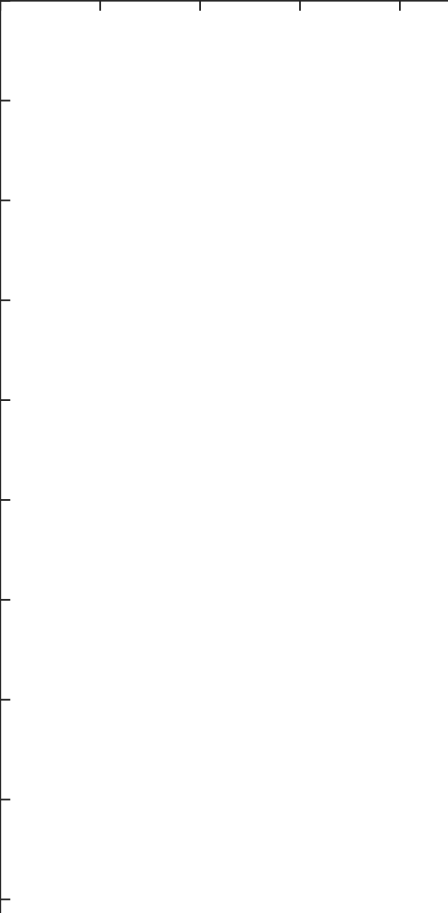
\includegraphics[width=0.2\textwidth]{Img/Experiment16_schemePlusAx.pdf}
}}
	\caption{Scheme of the measure scenario}
	\label{measureScheme}
\end{figure}

When playing the noise source signal only, the received signals by the microphones are shown in \autoref{recNS}. The spectrum has been calculated by applying the Fast Fourier Transform (FFT) to the received signal. The number of points used is the same as the number of samples of the signal, 1940400. The rest of spectra are calculated also in this way. An ideal response would present the same amplitude during the whole pulse. The real one presents significant variations due to the fact that the acoustic path response between loudspeaker and microphones is frequency selective. This is an indicator of the present multiple path phenomenon, diffractions, etc. The same type of variations are found in the received signal from the other loudspeakers. %(\autoref{recWFSexamp}).

\begin{figure}
	\begin{subfigure}[b]{0.49\textwidth}
		\centering
		\def\svgwidth{0.9\columnwidth}
		\graphicspath{{Img/}}
		{\fontsize{5}{12}\selectfont
			\input{Img/Experiment16_recNSTime.pdf_tex}
		}
		\caption{Time}
	\end{subfigure}
	\begin{subfigure}[b]{0.49\textwidth}
		\centering
		\def\svgwidth{0.9\columnwidth}
		\graphicspath{{Img/}}
		{\fontsize{5}{12}\selectfont
			\input{Img/Experiment16_recNSFreq.pdf_tex}
		}
		\caption{Frequency}
	\end{subfigure}
	\caption{Received signal from noise source}
	\label{recNS}
\end{figure}

When playing the noise source and WFS signals simultaneously, the received signals (in comparison with the ones received only from the noise source) are shown in \autoref{recSign}. As expected, no cancellation is achieved, since the real acoustic path responses $\AcPath[mat](f)$ are too different from the ideal ones.
\begin{figure}[h]
	\begin{subfigure}[b]{0.49\textwidth}
		\centering
		\def\svgwidth{0.9\columnwidth}
		\graphicspath{{Img/}}
		{\fontsize{5}{12}\selectfont
			\input{Img/Experiment16_recAndrecNStime_1.pdf_tex}
		}
		\caption{Time. Microphone 1.}
	\end{subfigure}
	\begin{subfigure}[b]{0.49\textwidth}
		\centering
		\def\svgwidth{0.9\columnwidth}
		\graphicspath{{Img/}}
		{\fontsize{5}{12}\selectfont
			\input{Img/Experiment16_recAndrecNStime_2.pdf_tex}
		}
		\caption{Time. Microphone 2.}
	\end{subfigure}
	\begin{subfigure}[b]{0.49\textwidth}
		\centering
		\def\svgwidth{0.9\columnwidth}
		\graphicspath{{Img/}}
		{\fontsize{5}{12}\selectfont
			\input{Img/Experiment16_recAndrecNSfreq_1.pdf_tex}
		}
		\caption{Frequency. Microphone 1.}
	\end{subfigure}
	\begin{subfigure}[b]{0.49\textwidth}
		\centering
		\def\svgwidth{0.9\columnwidth}
		\graphicspath{{Img/}}
		{\fontsize{5}{12}\selectfont
			\input{Img/Experiment16_recAndrecNSfreq_2.pdf_tex}
		}
		\caption{Frequency. Microphones 2.}
	\end{subfigure}
	\caption{Received signal}
	\label{recSign}
\end{figure}

It could be possible that noise cancellation was spoiled because there is a sound volume mismatch between the noise loudspeaker and the rest of loudspeakers.
Unlike the secondary array loudspeakers, which were all adjusted to have similar behaviour (same volume and response, though in reality there are of course inevitable variations), the noise loudspeaker volume can be independently adjusted manually by means of a potentiometer.
This introduces an unknown variable that definitely affects noise cancellation, even in the ideal model. Fortunately, this is relatively easy to model and compensate.

Basically, regarding the volume of the source as a separate variable when dealing with real loudspeakers, 
we transform \autoref{acPathModel} in:
\begin{equation}
\Field[noValue][frequency][vector]
= \soundVolume[ns]\AcPath[mat][NS]\vec{\signal[ns][frequency]}(f) + \soundVolume[wfs]\AcPath[mat][WFS]\vec{\signal[wfs][frequency]}(f),
\end{equation}
where $\soundVolume[ns]$ and $\soundVolume[wfs]$ are scalar real numbers that represent the volume of the noise and the secondary loudspeakers respectively.

In order to perform cancellation, we must compensate for this volume difference by multiplying the amplitude of secondary signals by $\globalCorrectionFactor = \soundVolume[ns]/\soundVolume[wfs]$. It could be estimated in different ways. A simple one is measuring the field generated by the noise loudspeaker and the secondary array separately. The result are two acoustic pressure signals for each microphone: ${\Field[ns][time]}(t)$ and ${\Field[wfs][time]}(t)$. Then, we must minimize the energy of the sum of both signals:
\begin{equation}
\globalCorrectionFactor = \min_{\correctionFactor} \int (\Field[wfs][time](t)\correctionFactor + \Field[ns][time](t))^2 \dif t.
\end{equation}

In reality, this signals are actually discrete vectors with as many elements as recorded samples (${\Field[wfs][time][vector]} [n]$ and ${\Field[ns][time][vector]} [n]$, where $n$ is the index of the sample). Hence, previous optimization becomes a simple vector operation.
\begin{equation}
\globalCorrectionFactor = \min_{\correctionFactor} \norm{\Field[wfs][time][vector]\correctionFactor + \Field[ns][time][vector]}^2 = -\frac{\scalarProd{\Field[wfs][time][vector]}{\Field[ns][time][vector]}}
{\norm{\Field[wfs][time][vector]}^2}.
\end{equation}
Let's notice that this estimation get's a value for each microphone. As we already know that for low frequencies cancellation is not good even in simulated scenarios, and that above the spatial aliasing frequency the synthesis is not correct, we have optimized considering just the interval that transmits frequencies between $500\si{Hz}$ and $850\si{Hz}$.
In \autoref{corrVol} there is the resulting signal after volume correction (the result is similar for the other microphone). The total signal is actually very similar to the contribution from just the noise source. This is not strange if we take in account that the volume correction factor we have applied is very small ($\globalCorrectionFactor = 0.1518$), so the contribution from the secondary array is minimal. What seems to have happened is that the correlation between $\Field[wfs][time][vector]$ and $\Field[ns][time][vector]$ is too small. In the ideal scenario, the correlation coefficient would be very close to one, so the estimated value would actually very close to $\soundVolume[ns]/\soundVolume[wfs]$. However, both variables are so uncorrelated that the best way of minimizing the total power of the sum of both is making the secondary signals very small. This means that the cause of the low cancellation levels is not the volume mismatch, but probably a combination of previously mentioned phenomena (reverberation, diffractions, irregular directivity patterns, etc.).

\begin{figure}[h]
	\centering
	\begin{subfigure}[b]{0.49\textwidth}
		\def\svgwidth{0.9\columnwidth}
		\graphicspath{{Img/}}
		{\fontsize{5}{12}\selectfont
			\input{Img/Experiment16_recAndrecNStimeCorrVolTime_1.pdf_tex}
		}
		\caption{Time}
	\end{subfigure}
	\begin{subfigure}[b]{0.49\textwidth}
		\def\svgwidth{0.9\columnwidth}
		\graphicspath{{Img/}}
		{\fontsize{5}{12}\selectfont
			\input{Img/Experiment16_recAndrecNSfreqCorrVolTime_1.pdf_tex}
		}
	\caption{Frequency}	
	\end{subfigure}
\caption{Received signal after volume correction. Microphone 1. $\globalCorrectionFactor = 0.1518$.}
	\label{corrVol}
\end{figure}